\setauthorname{Lukas Schachinger}

% Das ist nur Beispiel was wir schreiben könnten
\pagebreak
\section{Planung und Konzeption des Spiels}
\subsection{Story und Theme:}
\begin{enumerate}
  \item Vorstellung der Spielidee und des Storykonzepts.
  \item Beschreibung der Hintergrundgeschichte und Charaktere.
  \item Erklärung des gewählten Spielthemas und seiner Relevanz für die Spielerfahrung.
\end{enumerate}

\subsection{Leveldesign:}
\begin{enumerate}
  \item Einführung in das Leveldesign und seine Bedeutung für das Spielerlebnis.
  \item Beschreibung der geplanten Level, ihrer Ziele und Herausforderungen.
  \item Eventuell Skizzen oder Diagramme, die die Levelstruktur verdeutlichen.
\end{enumerate}

\subsection{UI-Design und User Experience:}
\begin{enumerate}
  \item Beschreibung des geplanten User Interfaces und dessen Funktionen (z. B. HUD, Menüs).
  \item Erklärung der gestalterischen Entscheidungen und UI-Elemente (z. B. Symbole, Farben).
  \item Diskussion der User Experience und wie sie das Gameplay beeinflusst.
\end{enumerate}

\subsection{Gameobjekte und deren Platzierung:}
\begin{enumerate}
  \item Vorstellung der verschiedenen Gameobjekte im Spiel und ihrer Funktionen.
  \item Diskussion der Platzierung und Verteilung der Gameobjekte in den Leveln.
  \item Erklärung, wie die Gameobjekte mit der Spielmechanik interagieren.
\end{enumerate}

\subsection{Spielanleitung und Steuerung:}
\begin{enumerate}
  \item Erstellung einer detaillierten Spielanleitung für die Spieler.
  \item Beschreibung der Steuerungsmöglichkeiten und Interaktionsmechanismen.
  \item Eventuell Integration von Tutorials oder Hilfestellungen für neue Spieler.
\end{enumerate}

% todo: remove this
\todo{remove this...}

\chapter{User Interface (UI) und Interaktion}

\begin{quote}
\emph{\glqq Im Interface begegnet der Spieler dem Spiel. [...] Die Schnittstelle zwischen Mensch und Computer/Konsole etc.\grqq}~\cite[p.~161]{GameDesign} \\
\end{quote}

Das UI im Spieldesign ist fast der wichtigste Teil der Spielentwicklung, wenn man das Design des eigentlichen Spieles außen vornimmt. 
Ohne eine gute Menu führung und ein gut entworfenes User Interface ist es schwer, dass Spielerinnen und Spieler das Spiel verstehen und spielen können. 

\begin{figure}[H]
  \centering
  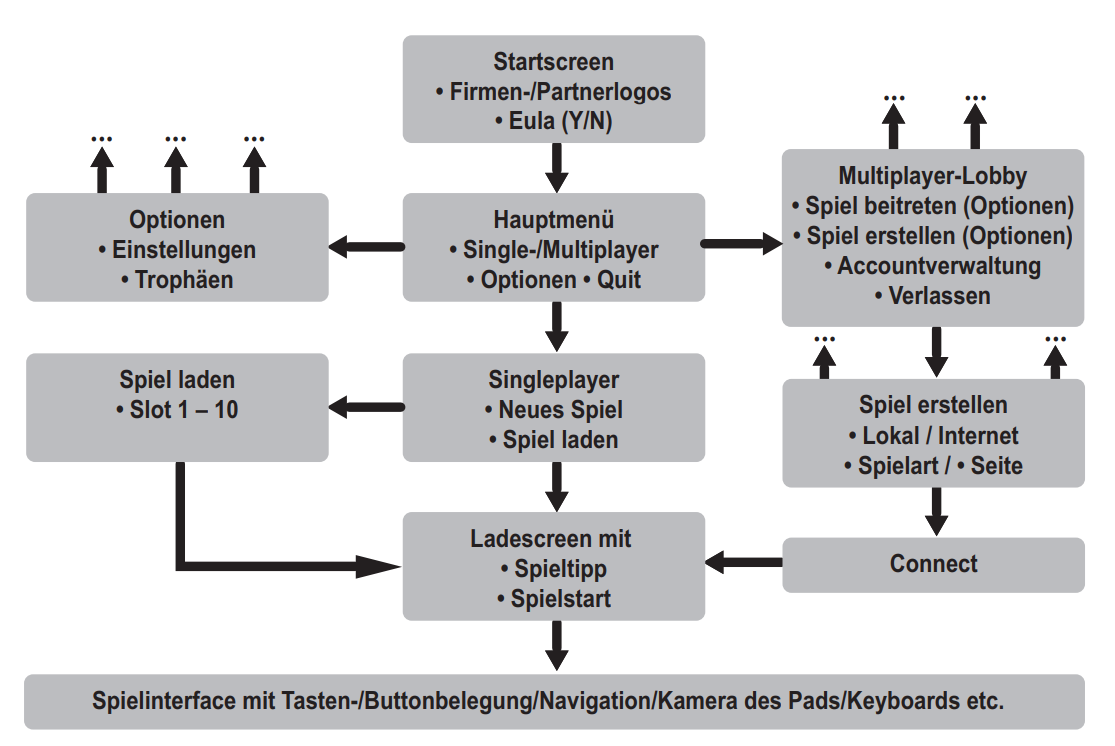
\includegraphics[width=0.8\textwidth]{chapters/03/images/Spielinterface.png}
  \caption{Ein Beispiel eines Dialogbaumes von einem Computerspiel.}
  \label{htl01}
\end{figure}

Der abgebildete Dialogbaum zeigt die verschiedenen Menüs und Screens die ein Computerspiel haben kann.
Diese unterscheiden sich in den unterschiedlichen Arten von Spielen. 
Bei einem \gls{multiplayer} Spiel soll die Möglichkeit geboten werden ein Spiel zu erstellen oder einem beizutreten. 
Während es bei einem \gls{singleplayer} wichtig ist Spielstände zu speichern und zu laden.

\pagebreak

Das \gls{UI} des Prototyps unterteilt sich in 3 verschiedene Aspekte:

\begin{itemize}
    \item Das Hauptmenü.
    \item Das \gls{UI} während des Spieles.
    \item Das Pause Menu.
\end{itemize}

\noindent
Bei der Entscheidung, welche Komplexität das User Interface des Prototyps haben soll, fiel die Wahl auf ein simples Design. 
Das \gls{UI} soll einerseits die Schlichtheit des eigentlichen Spieles wiederspiegeln und andererseits alle für das Spiel wichtigen Informationen darstellen.

\section{Gestaltung des Hauptmenüs}

Im Folgenden wird das Gestalten der Benutzeroberfläche für das Hauptmenü erläutert. 
Das Hauptmenü in der Spielentwicklung ist vergleichbar mit einem Türvorleger vor einer Haustür. Es soll das Willkommenschild für das eigentliche Spiel sein. 
Mithilfe dieses ersten Eindrucks ist es möglich zu erkennen um welche Art von Spiel es sich handelt. Das \gls{theme} des Spieles spiegelt sich in dem Design des Hintergrundes und in der Schriftart des Hauptmenüs wieder. Die Komplexität steht bei vielen Spielen in direkter Korrelation mit der Anzahl an Einstellungen in dem Hauptmenü.

\pagebreak

\subsection{Das Hauptmenü des Prototyps}

Das Hauptmenü des Prototyps besteht aus mehreren Komponenten. Die Hauptkomponente ist ein \gls{canvas}. Diesem untergeordnet ist ein Bild, ein \gls{gameObject} für das Hauptmenü und ein \gls{gameObject} für das Optionsmenü. Diese beiden GameObjecte sind die eigentlichen Menüs die dementsprechen ein- und ausgeblendet werden. Die Knöpfe die der User betätigen kann sind den Gameobjecten für das Hauptmenü und dem Optionsmenü untergeordnet. 
\subsubsection{Der Hintergrund}
Der Hintergrund des Hauptmenüs ist ein PNG von der \gls{skybox} des Spiels. 

\subsubsection{Die Buttons}
Die unten abgebildeten Abbildungen zeigen das Hauptmenü (links) und das Optionsmenü (rechts) des Prototyps. In dem Hauptmenü gibt es drei verschiedene Buttons: Play, Options and Quit. Play startet den Spielablauf, Options öffnet das Optionsmenü und Quit schließt das Spiel.\\\\
In dem Optionsmenü befindet sich die Lautstärkenregelung und... \\
Der "Back" Button um zurück in das Hauptmenü zu kommen befindet sich an letzter Stelle des Optionsmenüs.


\begin{figure}[H]
    \centering
    \begin{minipage}{0.4\textwidth}
        \centering
        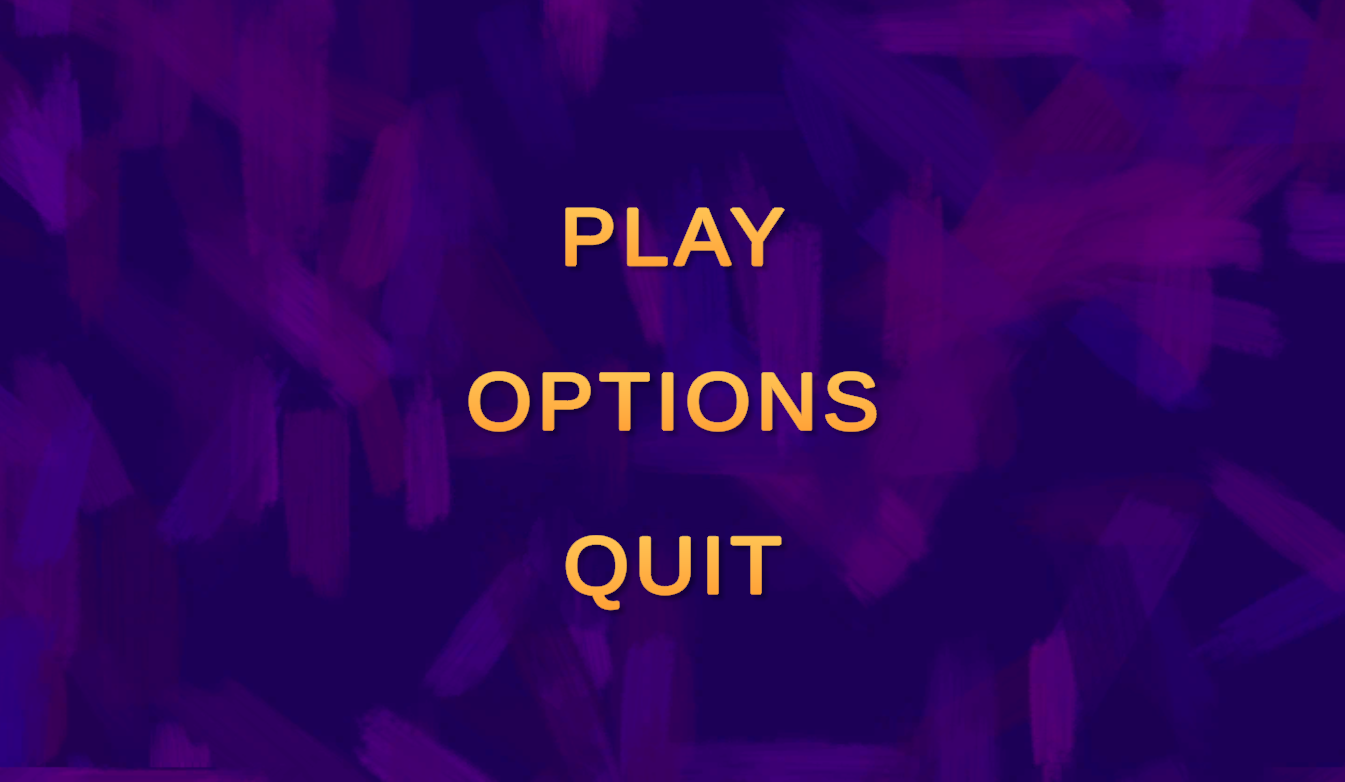
\includegraphics[width=\linewidth]{chapters/03/images/MainMenu.png}
        \caption{Das Hauptmenü des Prototyps.}
        \label{htl02a}
    \end{minipage}%
    \hspace{1cm}% Adjust the space here as needed
    \begin{minipage}{0.4\textwidth}
        \centering
        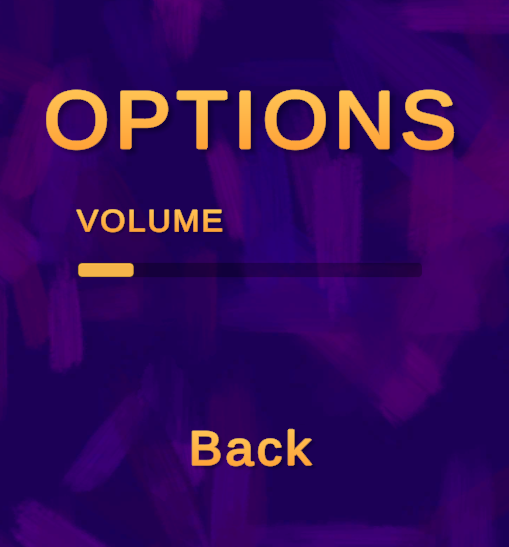
\includegraphics[width=\linewidth]{chapters/03/images/OptionsMainMenu.png}
        \caption{Das Optionsmenü des Prototyps.}
        \label{htl02b}
    \end{minipage}
\end{figure}

\section{Code behind des Menüs}

Der \gls{code-behind} des Menüs ist sehr simpel gehalten und auch einfach zu verstehen.

% C#
\begin{lstlisting}[language=CSharp,caption={Main Menu Klasse.},label=code:mainmenu]
public class MainMenu : MonoBehaviour
{
    public void PlayGame()
    {
        var activeScene = SceneManager.GetActiveScene();
        SceneManager.LoadScene(activeScene.buildIndex + 1);
    }

    public void QuitGame()
    {
        Debug.Log("Quit");
        Application.Quit();
    }
}
\end{lstlisting}
Der SceneManager ist ein einfacher Weg mittels einer Art von \gls{statemachine} eine Menüführung aufzubauen. In der nächsten Abbildung wird die Build-Reihenfolge der Scenes dargestellt.

\begin{center}
    \begin{figure}[h]
        \centering
        \includegraphics*[width=1\textwidth]{chapters/03/images/SceneManager.png}
        \caption{Der SceneManager in den Build Settings.}
        \label{htl04}
    \end{figure}
\end{center}

\noindent
Mittels der Code Zeile: 
% C#
\begin{lstlisting}[language=CSharp]
    SceneManager.LoadScene(activeScene.buildIndex + 1);
\end{lstlisting}
kann von der Menü Scene, die an der Stelle 0 ist zu der Projekt Scene, die an der Stelle 1 ist, gewechselt werden.

\pagebreak

\subsection{Die Funktion dem Button zuordnen}

In der nächsten Abbildung ist ein Ausschnitt der Properties des Play Buttons zu sehen. Bei der \verb+On Click ()+ Property wurde das \verb+MainMenu+ Script hinzugefügt. Nachdem das Script dort ausgewählt wurde, ist es möglich Methoden von diesem als Aktion für den Button auszuwählen. 

\begin{center}
    \begin{figure}[H]
        \centering
        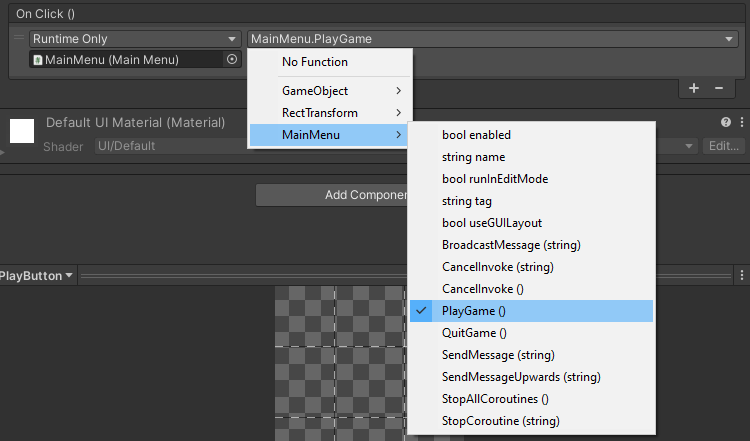
\includegraphics[width=1\textwidth]{chapters/03/images/PlayButton.png}
            \caption{Abbildung der Properties des Play Buttons.}
            \label{htl05}
    \end{figure}
\end{center}


\section{Game UI und Spielmechanik-Anzeigen}

\begin{figure}[H]
    \centering
    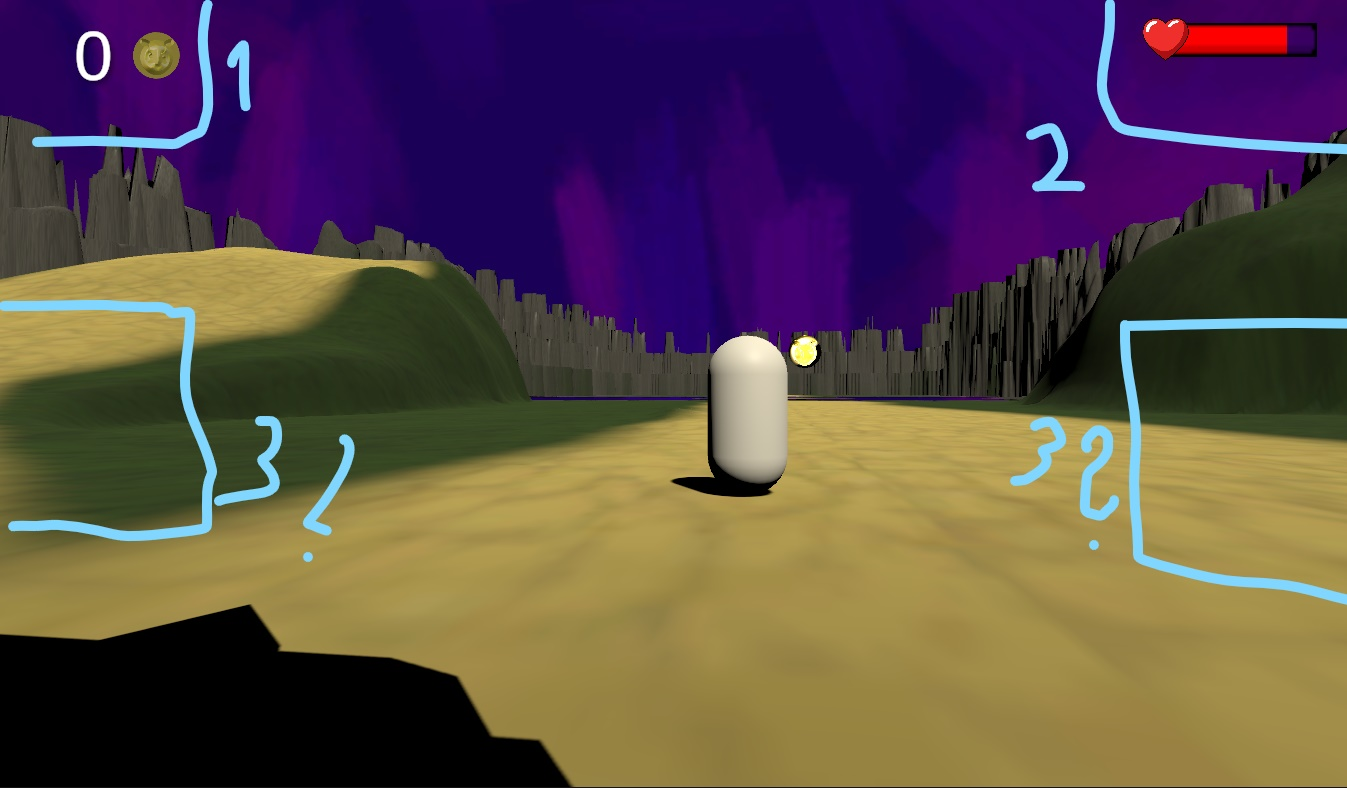
\includegraphics[width=1\textwidth]{chapters/03/images/InkedGameUI.jpg}
    \caption{Das UI während des Spiels.}
    \label{htl03}
\end{figure}

\subsection{Eulenmünzen (1)}
Sammelobjekte, oder auch Collectibles gennant, gibt es in vielen Computerspielen. Jedoch bieten sie die unterschiedlichsten Funktionen. In PacMan ist das Sammeln von den Punkten teil des Spielziels. Verglichen zu Donkey Kong, wo das Sammeln von den Collectibles nicht verpflichtend ist. Aber es ist Teil von 101\% Vervollständigung des Spiels.
%https://donkeykong.fandom.com/wiki/Donkey_Kong_64#Gameplay

Als Sammelobject gibt es in dem Prototypen so gennante \glqq Eulenmünzen\grqq. Diese dienen ähnlich wie bei Donkey Kong als nicht verpflichtende Nebenaufgabe. Die Münzen schweben überall verstreut über die Welt des Prototypen. 

\subsection{Lebensanzeige (2)}

Eine Lebensanzeige in einem Computerspiel ist ein dezenter Hinweis darauf, dass der Spielcharakter sterblich ist. Schaden kann von Gegnern oder Fallen genommen werden.

In dem Prototypen wird die Lebensanzeige als roter Balken neben einem Herz dargestellt. Dieses Symbol befindet sich in der rechten oberen Ecke des Bildschirms. Lebensenergie wird abgezogen wenn die Spielfigur von einem Gegner getroffen wird oder in das Void\footnote[1]{Das Void ist die Dunkelheit unter der Spielwelt.} fällt.

\subsection{Steuerung (3)}

Eine Darstellung der Steuerung auf dem User Interface ist ein einfacher Weg, das Spielkonzept dem Spieler näherzubringen. Ein gutes Beispiel dafür ist die Startwelt von Super Mario Odyssey. Dieses Spiel war auch eine große Inspiration für den Prototypen. 

\section{Optionen und Einstellungen}

% todo: continue this when ui better
\todo{Tbd...}

\section{Pause-Funktion und Benutzerfreundlichkeit}
Die Pause-Funktion ist ein wichtiger Teil eines Spiels. 

% todo: continue this
\todo{continue this?}

\begin{figure}[H]
  \centering
  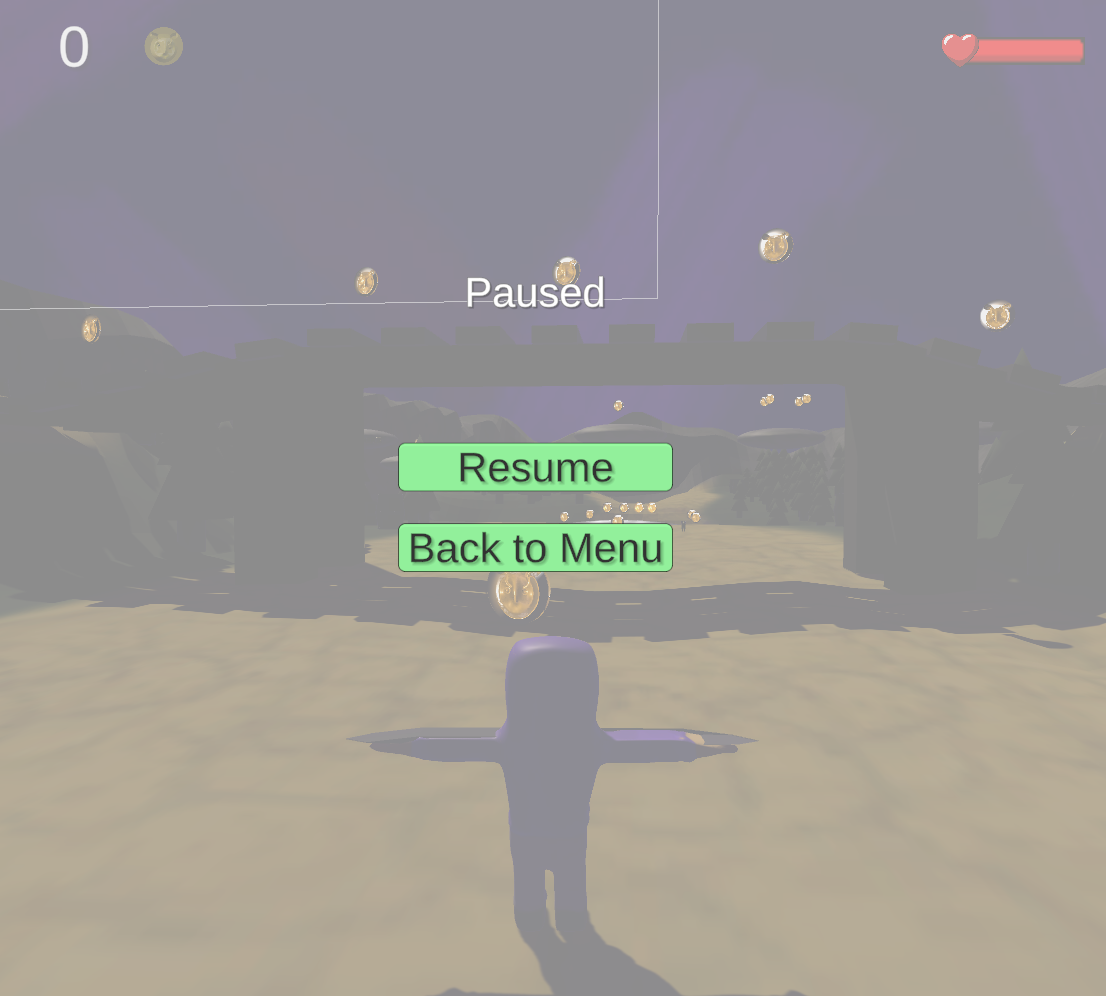
\includegraphics[width=0.5\textwidth]{chapters/03/images/GamePaused.png}
  \caption{Das Game Paused UI des Prototypen.}
  \label{luk01}
\end{figure}